\begin{figure}[!t]
\centering
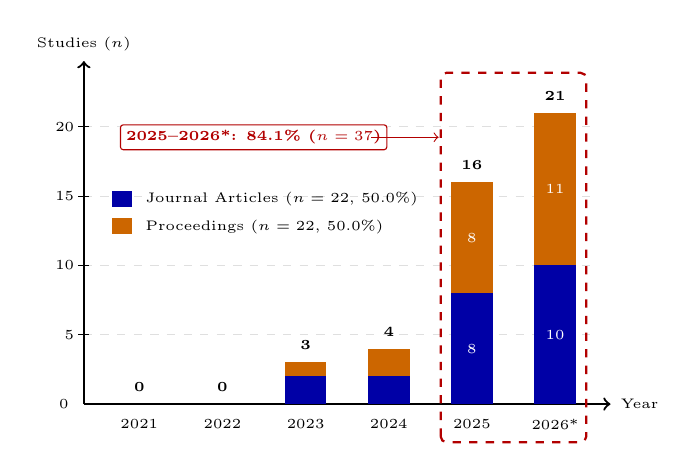
\begin{tikzpicture}[scale=0.88, font=\scriptsize]
  % Axes
  \draw[->, thick] (0,0) -- (7.6,0) node[right, font=\tiny] {Year};
  \draw[->, thick] (0,0) -- (0,4.95) node[above, font=\tiny] {Studies ($n$)};

  % Horizontal gridlines and y-ticks (scale: 1 unit = 5 articles -> y = n/5)
  \foreach \y/\lbl in {1/5, 2/10, 3/15, 4/20} {
    \draw[gray!25, dashed] (0,\y) -- (7.3,\y);
    \draw (-0.08,\y) -- (0.08,\y) node[left=2pt, font=\tiny] {\lbl};
  }
  \node[left=2pt, font=\tiny] at (0,0) {0};

  % Stacked bars: (x, journal_n, proc_n, total_lbl, year_lbl)
  % 2021: 0, 0
  \node[below=2pt, font=\tiny] at (0.8,0) {2021};
  \node[above=1pt, font=\tiny\bfseries] at (0.8,0) {0};

  % 2022: 0, 0
  \node[below=2pt, font=\tiny] at (2.0,0) {2022};
  \node[above=1pt, font=\tiny\bfseries] at (2.0,0) {0};

  % 2023: J=2 (0.4), P=1 (0.2), Total=3 (0.6)
  \fill[blue!65!black] (2.9,0) rectangle (3.5,0.4);
  \fill[orange!80!black] (2.9,0.4) rectangle (3.5,0.6);
  \node[below=2pt, font=\tiny] at (3.2,0) {2023};
  \node[above=1pt, font=\tiny\bfseries] at (3.2,0.6) {3};

  % 2024: J=2 (0.4), P=2 (0.4), Total=4 (0.8)
  \fill[blue!65!black] (4.1,0) rectangle (4.7,0.4);
  \fill[orange!80!black] (4.1,0.4) rectangle (4.7,0.8);
  \node[below=2pt, font=\tiny] at (4.4,0) {2024};
  \node[above=1pt, font=\tiny\bfseries] at (4.4,0.8) {4};

  % 2025: J=8 (1.6), P=8 (1.6), Total=16 (3.2)
  \fill[blue!65!black] (5.3,0) rectangle (5.9,1.6);
  \fill[orange!80!black] (5.3,1.6) rectangle (5.9,3.2);
  \node[white, font=\tiny] at (5.6,0.8) {8};
  \node[white, font=\tiny] at (5.6,2.4) {8};
  \node[below=2pt, font=\tiny] at (5.6,0) {2025};
  \node[above=1pt, font=\tiny\bfseries] at (5.6,3.2) {16};

  % 2026 YTD: J=10 (2.0), P=11 (2.2), Total=21 (4.2)
  \fill[blue!65!black] (6.5,0) rectangle (7.1,2.0);
  \fill[orange!80!black] (6.5,2.0) rectangle (7.1,4.2);
  \node[white, font=\tiny] at (6.8,1.0) {10};
  \node[white, font=\tiny] at (6.8,3.1) {11};
  \node[below=2pt, font=\tiny] at (6.8,0) {2026*};
  \node[above=1pt, font=\tiny\bfseries] at (6.8,4.2) {21};

  % Highlight bracket for 2025-2026 surge
  \draw[red!70!black, thick, dashed, rounded corners=2pt] (5.15,-0.55) rectangle (7.25,4.78);
  \node[fill=white, draw=red!70!black, rounded corners=1pt, font=\tiny\bfseries, text=red!70!black, inner sep=2pt] at (2.45,3.85) {2025--2026*: 84.1\% ($n=37$)};
  \draw[->, red!70!black, thin] (4.15,3.85) -- (5.12,3.85);

  % Legend
  \fill[blue!65!black] (0.4,2.85) rectangle (0.7,3.08);
  \node[right, font=\tiny] at (0.75,2.96) {Journal Articles ($n=22$, 50.0\%)};
  \fill[orange!80!black] (0.4,2.45) rectangle (0.7,2.68);
  \node[right, font=\tiny] at (0.75,2.56) {Proceedings ($n=22$, 50.0\%)};
\end{tikzpicture}
\caption{Annual publication trajectory of the validated corpus ($N=44$) disaggregated by publication venue type. *2026 reflects year-to-date Crossref indexing through November 10, 2026.}
\label{fig:temporal_distribution}
\end{figure}
